\documentclass{standalone}

\usepackage{amsmath}
\usepackage{tikz}
\usetikzlibrary{positioning}
\usepackage{pgfplots}
\pgfplotsset{compat=1.16}
\definecolor{BAMred1}{cmyk}{0.10, 1.00, 1.00, 0.00}
\definecolor{BAMred2}{cmyk}{0.30, 1.00, 1.00, 0.00}
\definecolor{BAMred3}{cmyk}{0.25, 1.00, 1.00, 0.35}
\definecolor{BAMblue1}{cmyk}{1.00, 0.00, 0.00, 0.00}
\definecolor{BAMblue2}{cmyk}{1.00, 0.40, 0.35, 0.25}
\definecolor{BAMblue3}{cmyk}{0.75, 0.00, 0.00, 0.80}
\definecolor{BAMblue4}{cmyk}{1.00, 0.70, 0.40, 0.70}
\definecolor{BAMyellow1}{cmyk}{0.00, 0.10, 1.00, 0.00}
\definecolor{BAMyellow2}{cmyk}{0.00, 0.25, 1.00, 0.15}
\definecolor{BAMyellow3}{cmyk}{0.00, 0.20, 1.00, 0.10}
\definecolor{BAMyellow4}{cmyk}{0.05, 0.40, 1.00, 0.20}
\definecolor{BAMgreen1}{cmyk}{0.20, 0.00, 1.00, 0.20}
\definecolor{BAMgreen2}{cmyk}{0.15, 0.00, 1.00, 0.50}
\definecolor{BAMgreen3}{cmyk}{0.75, 0.50, 1.00, 0.00}
\definecolor{BAMgreen4}{cmyk}{0.80, 0.60, 1.00, 0.50}
\definecolor{BAMgrad100}{cmyk}{0.45, 0.00, 0.00, 0.95}
\definecolor{BAMgrad080}{cmyk}{0.36, 0.00, 0.00, 0.76}
\definecolor{BAMgrad050}{cmyk}{0.225,0.00, 0.00, 0.475}
\definecolor{BAMgrad020}{cmyk}{0.09, 0.00, 0.00, 0.19}
\definecolor{BAMgrad010}{cmyk}{0.045, 0.00, 0.00, 0.095}


\begin{document}
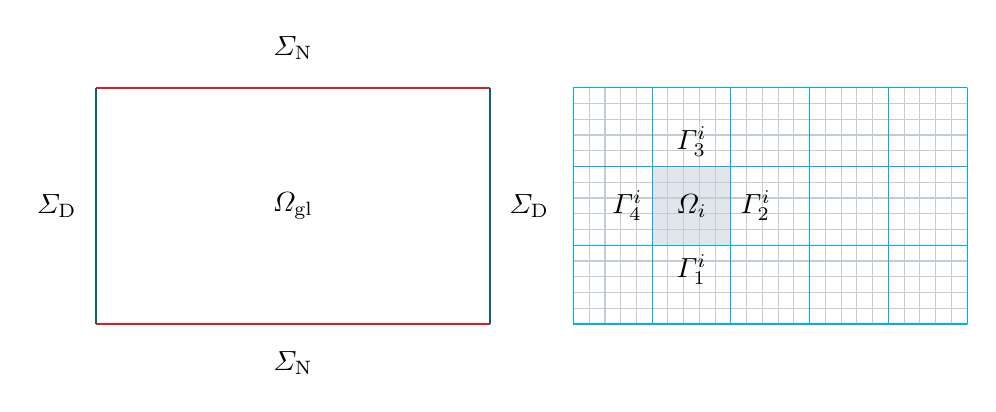
\begin{tikzpicture}
	\begin{scope}[xshift=-0.5 * \textwidth]
		\pgfmathsetmacro\w{5}
		\pgfmathsetmacro\h{0.6 * \w}
		\draw[BAMred1, thick] (0, 0) -- (\w, 0);
		\draw[BAMred1, thick] (0, \h) -- (\w, \h);
		\draw[BAMblue2, thick] (\w, 0) -- (\w, \h);
		\draw[BAMblue2, thick] (0, 0) -- (0, \h);
		% domain node
		\node at (\w / 2, \h / 2) {$\varOmega_{\mathrm{gl}}$};
		% dirichlet
		\coordinate (L) at (0, \h / 2);
		\path (L) ++(-0.5, 0) coordinate (LL);
		\node at (LL) {$\varSigma_{\mathrm{D}}$};
		\coordinate (R) at (\w, \h / 2);
		\path (R) ++(+0.5, 0) coordinate (RR);
		\node at (RR) {$\varSigma_{\mathrm{D}}$};
		% neumann
		\coordinate (B) at (\w / 2, 0);
		\path (B) ++(0, -0.5) coordinate (BB);
		\node at (BB) {$\varSigma_{\mathrm{N}}$};
		\coordinate (T) at (\w / 2, \h);
		\path (T) ++(0, +0.5) coordinate (TT);
		\node at (TT) {$\varSigma_{\mathrm{N}}$};
	\end{scope}
	\begin{scope}[xshift=0.0 * \textwidth]
		\pgfmathsetmacro\w{5}
		\pgfmathsetmacro\h{0.6 * \w}
		\pgfmathsetmacro\Nx{5}
		\pgfmathsetmacro\Ny{0.6 * \Nx}
		\pgfmathsetmacro\nx{25}
		\pgfmathsetmacro\ny{0.6 * \nx}
		% highlight subdomain
		\draw[fill, BAMgrad010] (\w / \Nx, \h / \Ny) coordinate (S) rectangle ++(\w / \Nx, \h / \Ny);
		% fine grid color
		\def\fc{BAMgrad020}
		\draw[\fc] (0, 0) rectangle (\w, \h);
		% vertical lines
		\foreach \x in {0, 1, 2, ..., \nx}{
			\draw[\fc] (\x / \nx * \w, 0.0)--(\x / \nx * \w, \h);
		}
		% horizontal lines
		\foreach \y in {0, 1, 2, ..., \ny}{
			\draw[\fc] (0, \y / \ny * \h)--(\w, \y / \ny * \h);
		}
		% coarse grid color
		\def\cc{BAMblue1}
		% vertical lines
		\foreach \x in {0, 1, 2, ..., \Nx}{
			\draw[\cc] (\x / \Nx * \w, 0.0)--(\x / \Nx * \w, \h);
		}
		% horizontal lines
		\foreach \y in {0, 1, 2, ..., \Ny}{
			\draw[\cc] (0, \y / \Ny * \h)--(\w, \y / \Ny * \h);
		}
		% annotate subdomain
		\path (S) ++(\w / \Nx / 2, \w / \Nx / 2) coordinate (Scenter);
		\node at (Scenter) {$\varOmega_i$};
		\node[below = \w / \Nx / 2 of Scenter] (bottom) {$\varGamma^i_1$};
		\node[right = \w / \Nx / 2 of Scenter] (right) {$\varGamma^i_2$};
		\node[above = \w / \Nx / 2 of Scenter] (top) {$\varGamma^i_3$};
		\node[left = \w / \Nx / 2 of Scenter] (left) {$\varGamma^i_4$};
	\end{scope}
\end{tikzpicture}
\end{document}
